\documentclass[12pt,a4paper]{article}

\usepackage{graphicx}
\usepackage{abstract}
\usepackage{wrapfig}
\usepackage{mathrsfs,amsmath} 
\usepackage{geometry}
\usepackage{fancyhdr}
\usepackage[T1]{fontenc}
\usepackage[polish]{babel}
\usepackage[utf8]{inputenc}
\usepackage{lmodern}
\usepackage{listings}
\usepackage{color}
\usepackage{xcolor}
\usepackage{hyperref}
\usepackage{subcaption}
\usepackage{multicol}
\usepackage{cleveref}
\usepackage{siunitx}

\setlength{\headheight}{12pt} 
\setlength{\textheight}{25cm}
\setlength{\textwidth}{17cm}
\setlength{\footskip}{10mm}
\setlength{\oddsidemargin}{0mm}
\setlength{\evensidemargin}{0mm}
\setlength{\topmargin}{0mm}
\setlength{\headsep}{10mm}

\lstdefinestyle{mystyle}{
    backgroundcolor=\color{backcolour},   
    commentstyle=\color{codegreen},
    keywordstyle=\color{magenta},
    numberstyle=\tiny\color{codegray},
    stringstyle=\color{codepurple},
    basicstyle=\footnotesize,
    breakatwhitespace=false,         
    breaklines=true,                 
    captionpos=b,                    
    keepspaces=true,                 
    numbers=left,                    
    numbersep=5pt,                  
    showspaces=false,                
    showstringspaces=false,
    showtabs=false,                  
    tabsize=2
}
 
\definecolor{codegreen}{rgb}{0,0.6,0}
\definecolor{codegray}{rgb}{0.5,0.5,0.5}
\definecolor{codepurple}{rgb}{0.58,0,0.82}
\definecolor{backcolour}{rgb}{0.95,0.95,0.92}
\lstset{style=mystyle}

\selectlanguage{polish}

\newgeometry{rmargin=2.5cm,lmargin=2.5cm,bmargin=2.5cm}
\pagestyle{fancy}
\rhead{Fizyka Techniczna}
\chead{}
\lhead{}
\lfoot{}
\cfoot{\thepage  }
\rfoot{}

\begin{document}

\thispagestyle{empty}
\begin{center}
{\Large \textbf{Fizyka Fazy Skondensowanej}}
\end{center}
\newpage

\tableofcontents
\newpage

\section{Zadania}
\subsection{Pierwszy}
\subsubsection{}
\begin{enumerate}
\item Sieć  krystaliczna, węzły sieci, proste sieciowe, płaszczyzny sieciowe, wskaźniki Millera (hkl), Komórka elementarna i  typy układów krystalograficznych
\item Operacje symetrii, grupy punktowe.
\item Sieć prosta a sieć odwrotna. Objętości komórki elementarnej w sieci odwrotnej. Odległości międzypłaszczyznowe. Strefy Brillouina.
\end{enumerate}

\subsubsection{}
Obliczyć objętość komórki elementarnej dla układu regularnego, romboedrycznego, heksagonalnego, jednoskośnego.
\subsubsection{}
Wykaż, że:
\begin{enumerate}
\item dla prostej sieci regularnej o stałej sieciowej $a$, odległość międzypłaszczyznowa \[d^2_{hkl} =\frac{a^2}{h^2+k^2+l^2}\] 
\item obliczyć $\frac{1}{d^2_{hkl}}$ dla układu heksagonalnego oraz rombowego
\end{enumerate}

\subsubsection{}
Struktura diamentu zawiera dwa identyczne atomy w położeniach $000$ i $\frac{1}{4}\frac{1}{4}\frac{1}{4}$ związane z każdym węzłem sieci powierzchniowo centrowanej \textit{(fcc)}. Obliczyć czynnik strukturalny dla tej struktury. Pokaż, że dozwolone odbicia spełniają warunek $h + k + l = 4n$, gdzie wszystkie wskaźniki są parzyste, a $n$ jest dowolna liczbą całkowitą, albo wszystkie składniki są nieparzyste.  

\newpage

\subsection{Drugi}
\subsubsection{}
Energia oddziaływania między dwoma atomami w cząsteczce opisywana jest wzorem:
\[U(r) = -\frac{\alpha}{r^n}+\frac{\beta}{r^m}\]
Pokazać, że $m>n$.
\subsubsection{}
Rozważ liniowy układ $2N$ jonów o ładunku równym na przemian $\pm q$. Załóż, że energia potencjalna odpychania między najbliższymi sąsiadami ma postać $\frac{A}{R^n}$. 
\begin{enumerate}
\item Pokaż, że dla odległości między jonami odpowiadającej stanowi równowagi 
\[U(R_0) = -\frac{2Nq^2\ln(2)}{R_0}\left(1-\frac{1}{n}\right)\]
\item Załóżmy, że kryształ został ściśnięty tak, że $R_0\rightarrow R_0(1-\delta)$. Pokaż, że w wyrażeniu na pracę związaną ze ściśnięciem kryształu największy wkład opisuje człon $\frac{C\delta^2}{2}$ gdzie:
\[C=\frac{(n-1)q^2\ln(2)}{R_0}\]
\end{enumerate}
\subsubsection{}
Obliczyć stałą Madelunga dla kryształu \textit{NaCl}:
\begin{enumerate}
\item przypadek jednowymiarowy (nić krystaliczna \textit{NaCl})
\begin{figure}[h!]
\centering
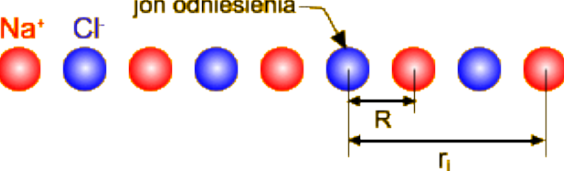
\includegraphics[scale=0.3]{images/zes2-1}
\end{figure}
\item przypadek dwuwymiarowy (siatka płaska \textit{NaCl})
\begin{figure}[h!]
\centering
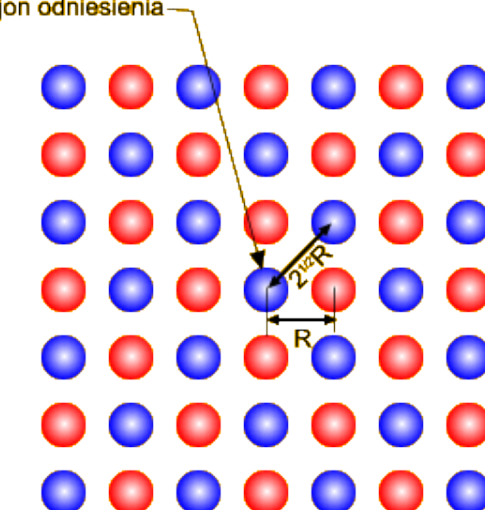
\includegraphics[scale=0.2]{images/zes2-2}
\end{figure}
\end{enumerate}
\subsubsection{}
Obliczyć jakie ciśnienie należy przyłożyć do kryształu jonowego, aby odległość między jonami zmniejszyła się o $1$ procent.

\listoffigures
\renewcommand{\lstlistingname}{Kod źródłowy}
\renewcommand{\lstlistlistingname}{\lstlistingname}
\lstlistoflistings

\end{document}
